% Standalone TikZ figure: fine-cell (K=4 x 368) multi-view retrieval encoder with a shared
% low-rank cell trunk and haversine label smoothing (T6/E3e, fold-0 screen 137.16km trained
% decode -> 132.72km swept decode, 2026-08-27). This is the LAST model of the geo-cell
% classification line -- the immediate predecessor of the convnextv2_femto pure-retrieval
% model that reached 59.22km pooled OOF (see best_result/README.md), which is a different
% architecture class entirely (no cells, no country head, no offset head).
%
% Kept as a separate file per this project's convention of not overwriting earlier
% architecture figures (see architecture_t3_4.tex / architecture_t4_1c.tex header notes).
% Builds directly on architecture_t4_1c.tex; the deltas from that figure are marked NEW.
%
% Compile alone:      tectonic architecture_t6_e3e.tex   (or pdflatex/lualatex/xelatex)
%
% All values below are read from the run's own artefacts, not from the working notes:
%   failed_experiments/_superseded_T2_to_T6/T6_E3e_cells368_hsmooth45_fold0/
%     config.json, param_compliance.json, fold0/fold_result.json, fold0/history.json,
%     eval_cv_sweep.json
%
% Delta vs T4.1c (architecture_t4_1c.tex), in the order they matter:
%   (1) NEW  cells 96 -> 368 per partition, K = 3 -> 4 partitions
%            (outputs/protocol/geo_cells_multi_fine)
%   (2) NEW  shared low-rank cell trunk Linear(1280->224)+GELU before the four cell heads;
%            without it 4 x (1280->368) alone would cost 1.89M params and blow the budget.
%   (3) NEW  haversine label smoothing (PIGEON, Haas et al. 2024) replaces the one-hot cell
%            target: tau = 45km. This is the single change that produced the first real win
%            (E3d, 148.5km); finer cells ALONE with one-hot targets were a wash (E3c, ~160km).
%   (4) NEW  orientation correction at the input (geo_dataset/orientation_flags.json).
%   (5)      embedding_dim 256 -> 224 (budget), EMA explicitly OFF (ema_decay 0.0),
%            trained from ImageNet init (init_checkpoint ""), 55 epochs, not warm-started.

\documentclass[tikz,border=4pt]{standalone}
\usepackage{amsmath}
\usetikzlibrary{positioning, arrows.meta, fit, backgrounds, shapes.geometric, calc}

\begin{document}
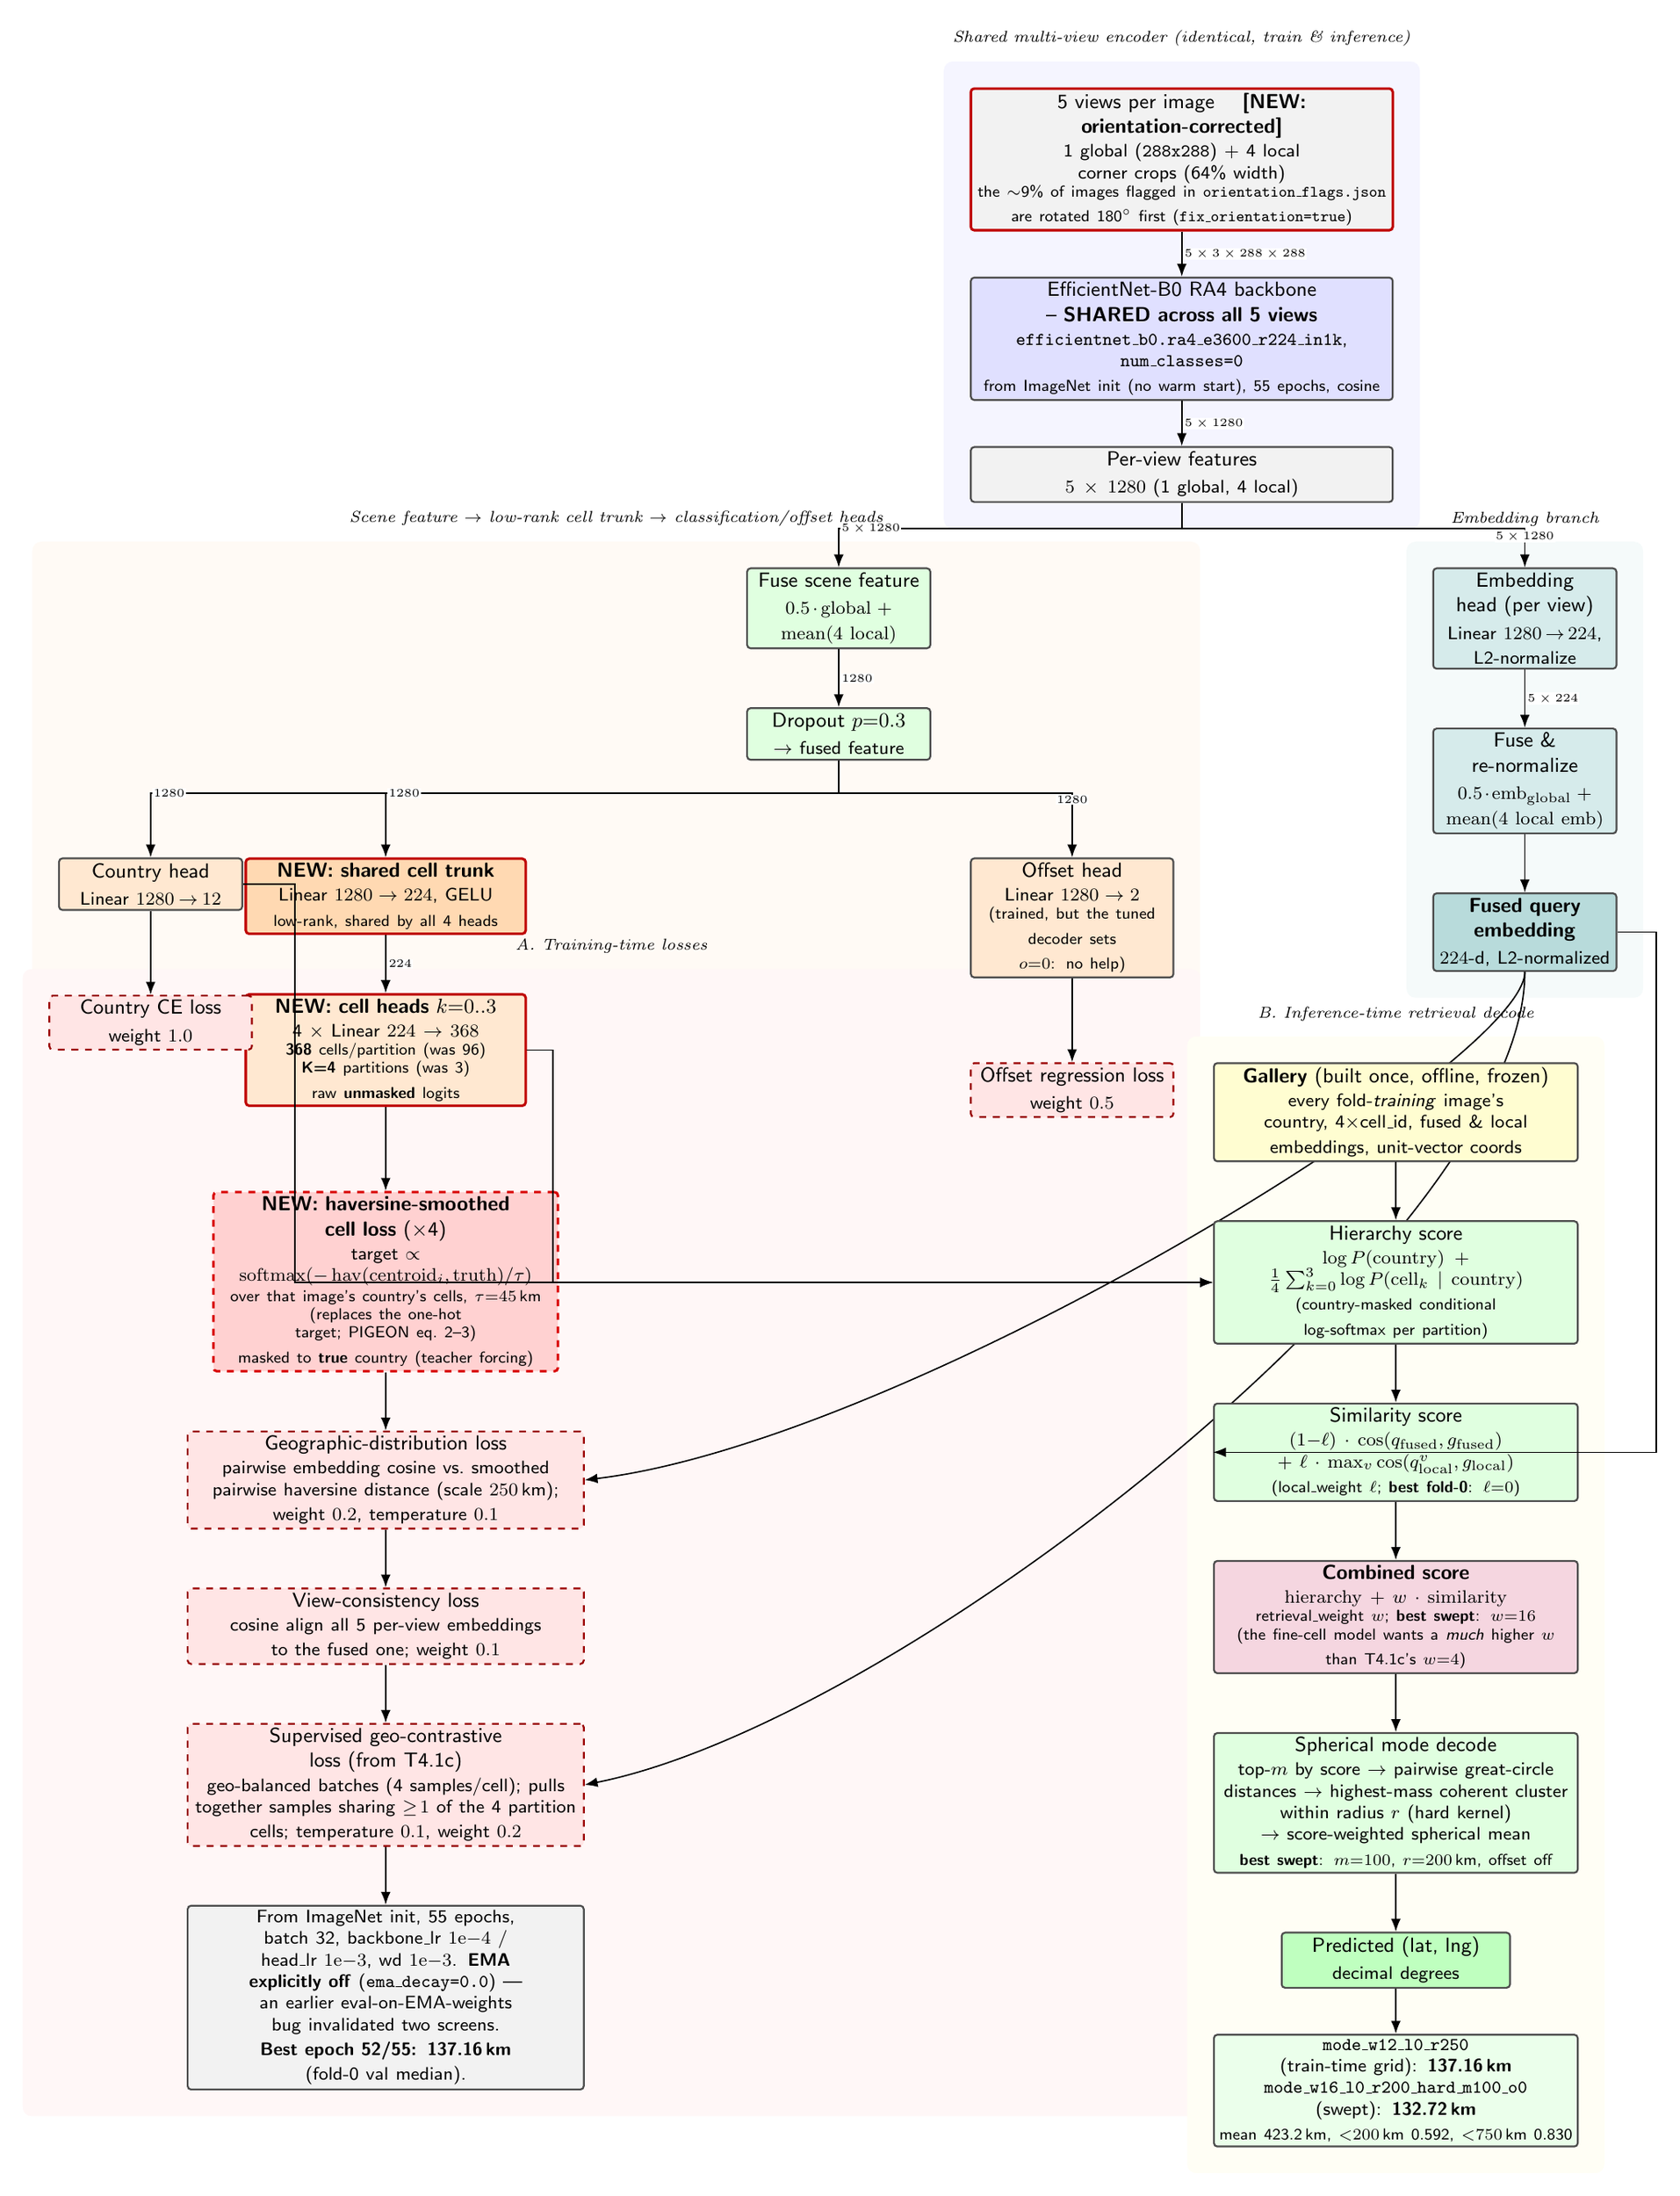
\begin{tikzpicture}[
  font=\sffamily\small,
  execute at begin picture={\hyphenpenalty=10000\exhyphenpenalty=10000\relax},
  node distance=7mm and 9mm,
  >={Latex[length=2mm,width=1.5mm]},
  every path/.style={line width=0.6pt},
  block/.style={
    rectangle, rounded corners=1.5pt, draw=black!70, thick,
    minimum height=8mm, text width=30mm, align=center, inner sep=2pt
  },
  backbone/.style={block, fill=blue!12, text width=64mm},
  head/.style={block, fill=orange!18, text width=27mm},
  emb/.style={block, fill=teal!16, text width=27mm},
  op/.style={block, fill=green!12, text width=27mm},
  fuse/.style={block, fill=purple!16, thick, text width=40mm},
  loss/.style={block, fill=red!10, dashed, draw=red!60!black, text width=30mm},
  gallery/.style={block, fill=yellow!18, text width=32mm},
  outnode/.style={block, fill=green!25, thick, text width=34mm},
  newbox/.style={draw=red!75!black, line width=1.1pt},
  dimlabel/.style={font=\tiny\itshape, pos=0.5, right=0.5pt, fill=white, inner sep=0.5pt},
  dimlabelb/.style={font=\tiny\itshape, pos=0.5, below=0.5pt, fill=white, inner sep=0.5pt},
]

% =========================================================================================
% SHARED ENCODER (identical at train and inference time)
% =========================================================================================
\node[block, fill=black!5, text width=64mm, newbox] (input)
  {5 views per image \quad\textbf{[NEW: orientation-corrected]}\\[1pt]
   \footnotesize 1 global (\texttt{288x288}) $+$ 4 local corner crops (64\% width)\\
   \scriptsize the $\sim$9\% of images flagged in \texttt{orientation\_flags.json}\\
   are rotated 180$^\circ$ first (\texttt{fix\_orientation=true})};
\node[backbone, below=of input] (backbone)
  {EfficientNet-B0 RA4 backbone -- \textbf{SHARED across all 5 views}\\[1pt]
   \footnotesize\texttt{efficientnet\_b0.ra4\_e3600\_r224\_in1k}, \texttt{num\_classes=0}\\
   \scriptsize from ImageNet init (no warm start), 55 epochs, cosine};
\draw[->] (input) -- (backbone) node[dimlabel]{$5\times3\times288\times288$};

\node[block, fill=black!5, below=of backbone, text width=64mm] (perview)
  {Per-view features\\[1pt]\footnotesize $5 \times 1280$ (1 global, 4 local)};
\draw[->] (backbone) -- (perview) node[dimlabel]{$5\times1280$};

% ---- split: scene-feature path (left) vs. embedding path (right) ----
\node[op, below left=10mm and 6mm of perview] (fuse_feat)
  {Fuse scene feature\\[1pt]\footnotesize $0.5\!\cdot\!\mathrm{global} + \mathrm{mean}(4\ \mathrm{local})$};
\node[emb, below right=10mm and 6mm of perview] (emb_head)
  {Embedding head (per view)\\[1pt]\footnotesize Linear $1280\!\to\!224$, L2-normalize};

\draw[->] (perview.south) -- ++(0,-4mm) -| (fuse_feat.north) node[pos=0.3,dimlabel]{$5\times1280$};
\draw[->] (perview.south) -- ++(0,-4mm) -| (emb_head.north) node[pos=0.7,dimlabelb]{$5\times1280$};

\node[op, below=9mm of fuse_feat] (dropout)
  {Dropout $p{=}0.3$\\[1pt]\footnotesize $\to$ fused feature};
\draw[->] (fuse_feat) -- (dropout) node[dimlabel]{$1280$};

\node[emb, below=9mm of emb_head] (fuse_emb)
  {Fuse \& re-normalize\\[1pt]\footnotesize $0.5\!\cdot\!\mathrm{emb}_{\mathrm{global}} + \mathrm{mean}(4\ \mathrm{local\ emb})$};
\draw[->] (emb_head) -- (fuse_emb) node[dimlabel]{$5\times224$};

\node[emb, below=9mm of fuse_emb, fill=teal!28, thick] (final_emb)
  {\textbf{Fused query embedding}\\[1pt]\footnotesize $224$-d, L2-normalized};
\draw[->] (fuse_emb) -- (final_emb);

% ---- heads off the fused 1280-d feature: country, low-rank trunk -> K=4 cell heads, offset
\node[head, below left=15mm and 78mm of dropout] (country_head)
  {Country head\\[1pt]\footnotesize Linear $1280\!\to\!12$};
\node[head, below left=15mm and 34mm of dropout, newbox, fill=orange!30, text width=42mm] (cell_proj)
  {\textbf{NEW: shared cell trunk}\\[1pt]\footnotesize Linear $1280\!\to\!224$, GELU\\
   \scriptsize low-rank, shared by all 4 heads};
\node[head, below right=15mm and 6mm of dropout, text width=30mm] (offset_head)
  {Offset head\\[1pt]\footnotesize Linear $1280\!\to\!2$\\
   \scriptsize (trained, but the tuned\\ decoder sets $o{=}0$: no help)};

\draw[->] (dropout.south) -- ++(0,-5mm) -| (country_head.north) node[pos=0.25,dimlabel]{$1280$};
\draw[->] (dropout.south) -- ++(0,-5mm) -| (cell_proj.north) node[pos=0.4,dimlabel]{$1280$};
\draw[->] (dropout.south) -- ++(0,-5mm) -| (offset_head.north) node[pos=0.75,dimlabelb]{$1280$};

\node[head, below=9mm of cell_proj, newbox, text width=42mm] (cell_heads)
  {\textbf{NEW: cell heads} $k{=}0..3$\\[1pt]\footnotesize 4 $\times$ Linear $224\!\to\!368$\\
   \scriptsize \textbf{368} cells/partition (was 96)\\ \textbf{K=4} partitions (was 3)\\
   raw \textbf{unmasked} logits};
\draw[->] (cell_proj) -- (cell_heads) node[dimlabel]{$224$};

% =========================================================================================
% A. TRAINING-TIME LOSSES
% =========================================================================================
\node[loss, below=13mm of country_head] (l_country)
  {Country CE loss\\[1pt]\footnotesize weight $1.0$};
\draw[->] (country_head) -- (l_country);

\node[loss, below=13mm of cell_heads, newbox, draw=red!85!black, fill=red!18, text width=52mm] (l_cell)
  {\textbf{NEW: haversine-smoothed cell loss} ($\times$4)\\[1pt]
   \footnotesize target $\propto\ \mathrm{softmax}\!\left(-\,\mathrm{hav}(\mathrm{centroid}_i, \mathrm{truth})/\tau\right)$\\[1pt]
   \scriptsize over that image's country's cells, $\tau{=}45$\,km\\
   (replaces the one-hot target; PIGEON eq.~2--3)\\
   \scriptsize masked to \textbf{true} country (teacher forcing)};
\draw[->] (cell_heads) -- (l_cell);

\node[loss, below=13mm of offset_head] (l_offset)
  {Offset regression loss\\[1pt]\footnotesize weight $0.5$};
\draw[->] (offset_head) -- (l_offset);

\node[loss, below=9mm of l_cell, text width=60mm] (l_geo)
  {Geographic-distribution loss\\[1pt]\footnotesize pairwise embedding cosine vs.\ smoothed\\
   pairwise haversine distance (scale $250$\,km);\\ weight $0.2$, temperature $0.1$};
\draw[->] (final_emb.south) .. controls +(0,-14mm) and +(50mm,6mm) .. (l_geo.east);
\draw[->] (l_cell) -- (l_geo);

\node[loss, below=9mm of l_geo, text width=60mm] (l_consist)
  {View-consistency loss\\[1pt]\footnotesize cosine align all 5 per-view embeddings\\
   to the fused one; weight $0.1$};
\draw[->] (l_geo) -- (l_consist);

\node[loss, below=9mm of l_consist, text width=60mm] (l_contrastive)
  {Supervised geo-contrastive loss (from T4.1c)\\[1pt]
   \footnotesize geo-balanced batches (4 samples/cell); pulls\\
   together samples sharing $\ge\!1$ of the 4 partition\\
   cells; temperature $0.1$, weight $0.2$};
\draw[->] (l_consist) -- (l_contrastive);
\draw[->] (final_emb.south) .. controls +(0,-40mm) and +(50mm,10mm) .. (l_contrastive.east);

\node[block, fill=black!5, below=9mm of l_contrastive, text width=60mm] (trainnote)
  {\footnotesize From ImageNet init, 55 epochs, batch 32, backbone\_lr $1\mathrm{e}{-4}$ /\\
   head\_lr $1\mathrm{e}{-3}$, wd $1\mathrm{e}{-3}$. \textbf{EMA explicitly off} (\texttt{ema\_decay=0.0}) ---\\
   an earlier eval-on-EMA-weights bug invalidated two screens.\\
   \textbf{Best epoch 52/55: 137.16\,km} (fold-0 val median).};
\draw[->] (l_contrastive) -- (trainnote);

% =========================================================================================
% B. INFERENCE-TIME RETRIEVAL DECODE
% =========================================================================================
\node[gallery, below right=13mm and 6mm of offset_head, text width=55mm] (gallery_build)
  {\textbf{Gallery} (built once, offline, frozen)\\[1pt]\footnotesize every fold-\emph{training} image's\\
   country, 4$\times$cell\_id, fused \& local\\ embeddings, unit-vector coords};

\node[op, below=9mm of gallery_build, text width=55mm] (hierarchy_score)
  {Hierarchy score\\[1pt]\footnotesize $\log P(\mathrm{country}) + \tfrac{1}{4}\sum_{k=0}^{3}\log P(\mathrm{cell}_k\!\mid\!\mathrm{country})$\\
   \scriptsize (country-masked conditional log-softmax per partition)};
\draw[->] (country_head.east) -- ++(8mm,0) |- (hierarchy_score.west);
\draw[->] (cell_heads.east) -- ++(4mm,0) |- (hierarchy_score.west);
\draw[->] (gallery_build) -- (hierarchy_score);

\node[op, below=9mm of hierarchy_score, text width=55mm] (sim_score)
  {Similarity score\\[1pt]\footnotesize $(1{-}\ell)\cdot\cos(q_{\mathrm{fused}}, g_{\mathrm{fused}})$
   $+\ \ell\cdot\max_v \cos(q^v_{\mathrm{local}}, g_{\mathrm{local}})$\\
   \scriptsize (local\_weight $\ell$; \textbf{best fold-0}: $\ell{=}0$)};
\draw[->] (final_emb.east) -- ++(6mm,0) |- (sim_score.west);
\draw[->] (hierarchy_score) -- (sim_score);

\node[fuse, below=9mm of sim_score, text width=55mm] (combined_score)
  {\textbf{Combined score}\\[1pt]\footnotesize $\mathrm{hierarchy} + w\cdot\mathrm{similarity}$\\
   \scriptsize retrieval\_weight $w$; \textbf{best swept}: $w{=}16$\\
   (the fine-cell model wants a \emph{much} higher $w$\\ than T4.1c's $w{=}4$)};
\draw[->] (sim_score) -- (combined_score);

\node[op, below=9mm of combined_score, text width=55mm] (mode_decode)
  {Spherical mode decode\\[1pt]\footnotesize top-$m$ by score $\to$ pairwise great-circle\\
   distances $\to$ highest-mass coherent cluster\\
   within radius $r$ (hard kernel)\\
   $\to$ score-weighted spherical mean\\
   \scriptsize \textbf{best swept}: $m{=}100$, $r{=}200$\,km, offset off};
\draw[->] (combined_score) -- (mode_decode);

\node[outnode, below=9mm of mode_decode] (final)
  {Predicted (lat, lng)\\[1pt]\footnotesize decimal degrees};
\draw[->] (mode_decode) -- (final);

\node[block, fill=green!8, below=7mm of final, text width=55mm] (resultnote)
  {\footnotesize \texttt{mode\_w12\_l0\_r250} (train-time grid): \textbf{137.16\,km}\\
   \texttt{mode\_w16\_l0\_r200\_hard\_m100\_o0} (swept): \textbf{132.72\,km}\\
   \scriptsize mean 423.2\,km, ${<}200$\,km 0.592, ${<}750$\,km 0.830};
\draw[->] (final) -- (resultnote);

% ---- background grouping boxes ----
% NOTE: group labels are plain foreground nodes anchored off each fit box's `.north`, not
% `fit`'s `label=` key -- see architecture_t4_1c.tex for why (bounding-box clipping).
\begin{scope}[on background layer]
  \node[fit=(input)(backbone)(perview), fill=blue!4, rounded corners=4pt, inner sep=4mm] (fit_encoder) {};
  \node[fit=(fuse_feat)(dropout)(country_head)(cell_proj)(cell_heads)(offset_head), fill=orange!4, rounded corners=4pt, inner sep=4mm] (fit_heads) {};
  \node[fit=(emb_head)(fuse_emb)(final_emb), fill=teal!4, rounded corners=4pt, inner sep=4mm] (fit_emb) {};
  \node[fit=(l_country)(l_cell)(l_offset)(l_geo)(l_consist)(l_contrastive)(trainnote), fill=red!3, rounded corners=4pt, inner sep=4mm] (fit_losses) {};
  \node[fit=(gallery_build)(hierarchy_score)(sim_score)(combined_score)(mode_decode)(final)(resultnote), fill=yellow!4, rounded corners=4pt, inner sep=4mm] (fit_decode) {};
\end{scope}

\node[font=\scriptsize\itshape, above=1mm of fit_encoder.north] {Shared multi-view encoder (identical, train \& inference)};
\node[font=\scriptsize\itshape, above=1mm of fit_heads.north] {Scene feature $\to$ low-rank cell trunk $\to$ classification/offset heads};
\node[font=\scriptsize\itshape, above=1mm of fit_emb.north] {Embedding branch};
\node[font=\scriptsize\itshape, above=1mm of fit_losses.north] {A. Training-time losses};
\node[font=\scriptsize\itshape, above=1mm of fit_decode.north] {B. Inference-time retrieval decode};

\end{tikzpicture}
\end{document}

% ---------------------------------------------------------------------------------------
% Params (from param_compliance.json / config.json "n_params_total"; the breakdown below
% is the arithmetic that reproduces that total exactly):
%   backbone (efficientnet_b0.ra4_e3600_r224_in1k, shared across all 5 views)   4,007,548
%   country head (1280->12)                                                       15,372
%   NEW shared cell trunk (1280->224, +GELU)                                     286,944
%   NEW cell heads k=0..3 (224->368 each, x4)                                    331,200
%   offset head (1280->2)                                                          2,562
%   embedding head (1280->224, shared across all 5 views)                        286,944
%   TOTAL                                                                      4,930,570   / 5,000,000 budget
%
% Note the point of the low-rank trunk: 4 x (1280->368) direct heads would cost 1,886,208
% params on their own. Trunk + heads together cost 618,144 -- a 1.27M saving, which is what
% makes K=4 x 368 cells fit under the 5M cap at all.
%
% fold-0 screen results (2026-08-27, best epoch 52 of 55):
%   country top-1 acc 0.783, cell top-1 acc 0.130 (368-way; deliberately low -- the smoothed
%   target flattens the argmax while keeping the DISTRIBUTION well-placed, which is what the
%   mode decode consumes. Compare E1's 0.43 cell acc at 96 cells and a WORSE 153.6km median.)
%   hard (cell-argmax, no retrieval) decode: 156.75km  vs  retrieval mode decode: 137.16km.
%
% Line progression on fold 0 (all EfficientNet-B0):
%   E1   96 cells,  K=4, one-hot                              153.6 km
%   E3c  192 cells, K=3, one-hot (finer cells ALONE)         ~160   km  (a wash)
%   E3d  192 cells, K=3, + haversine smoothing tau=65         148.5 km  (first win)
%   E3e  368 cells, K=4, + smoothing tau=45, low-rank trunk   137.2 km -> 132.7 km swept
%   E5   same recipe, folds 1 / 2                             135.3 / 138.0 km
%   4-model score-space fusion (E3e+E4+E3d+E3h)               122.3 km
% Superseded by the convnextv2_femto GeM retrieval model: 59.22km pooled OOF over all 5
% official folds (best_result/README.md) -- a different architecture class, not an increment
% on this one.
%
% Per-country fold-0 median km at the best swept decoder (eval_cv_sweep.json):
%   Iceland  52.0 | Belarus  84.5 | Finland  85.7 | Norway  95.6 | Turkey 112.5
%   Sweden  118.9 | UK      129.8 | Poland  204.8 | Germany 272.8 | Spain  311.4
%   Italy   362.9 | France  464.2
%   France/Italy/Spain are 25% of the fold and carry the error; the diagnosis at the time
%   was country-head misclassification (France country acc 0.585), which is precisely the
%   failure mode the later cell-free retrieval model avoids by having no country head.
% ---------------------------------------------------------------------------------------
